\documentclass{beamer}

% \usepackage{beamerthemesplit} // Activate for custom appearance
\usetheme{Boadilla}
%\setbeamertemplate{footline}[page number]{}
\usepackage{graphicx,subfig,float, xmpmulti, multicol, dsfont, hyperref}
\usepackage{bm} % for math bold
\usepackage{color} % font color

%draw neural network
\usepackage{tikz} 
\usetikzlibrary{matrix,chains,positioning,decorations.pathreplacing,arrows}



\begin{document}

%%%%%%%%%%%%%%%%%%%%%%%%%%%%%%%%%%%%%%%%%%%%%%%%%%%%

\frame{
\frametitle{Kaplan-Meier Estimate }
\centering
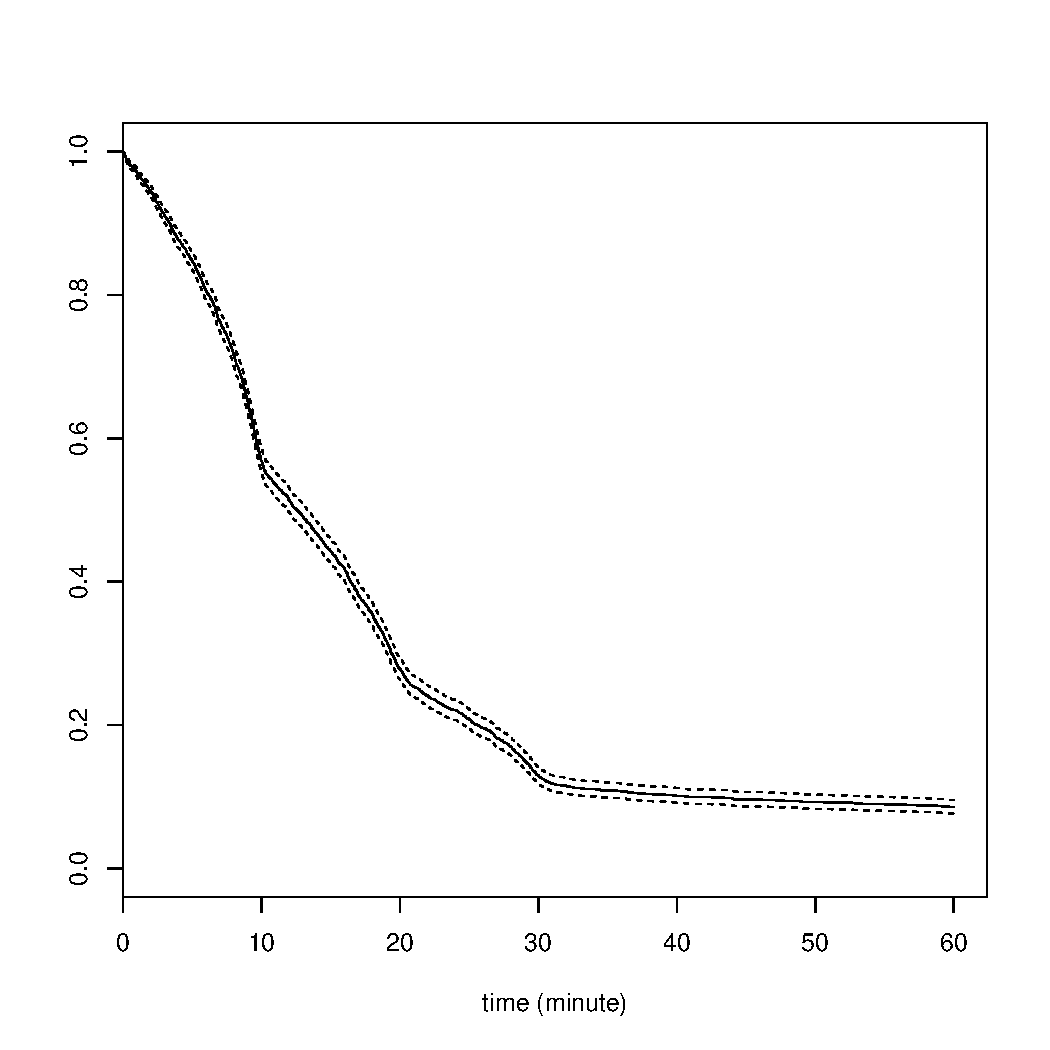
\includegraphics[width = .7\textwidth]{Figure/fig_KM.pdf}
}

\frame{
\frametitle{Kaplan-Meier Estimate with Different Article Class}
\centering
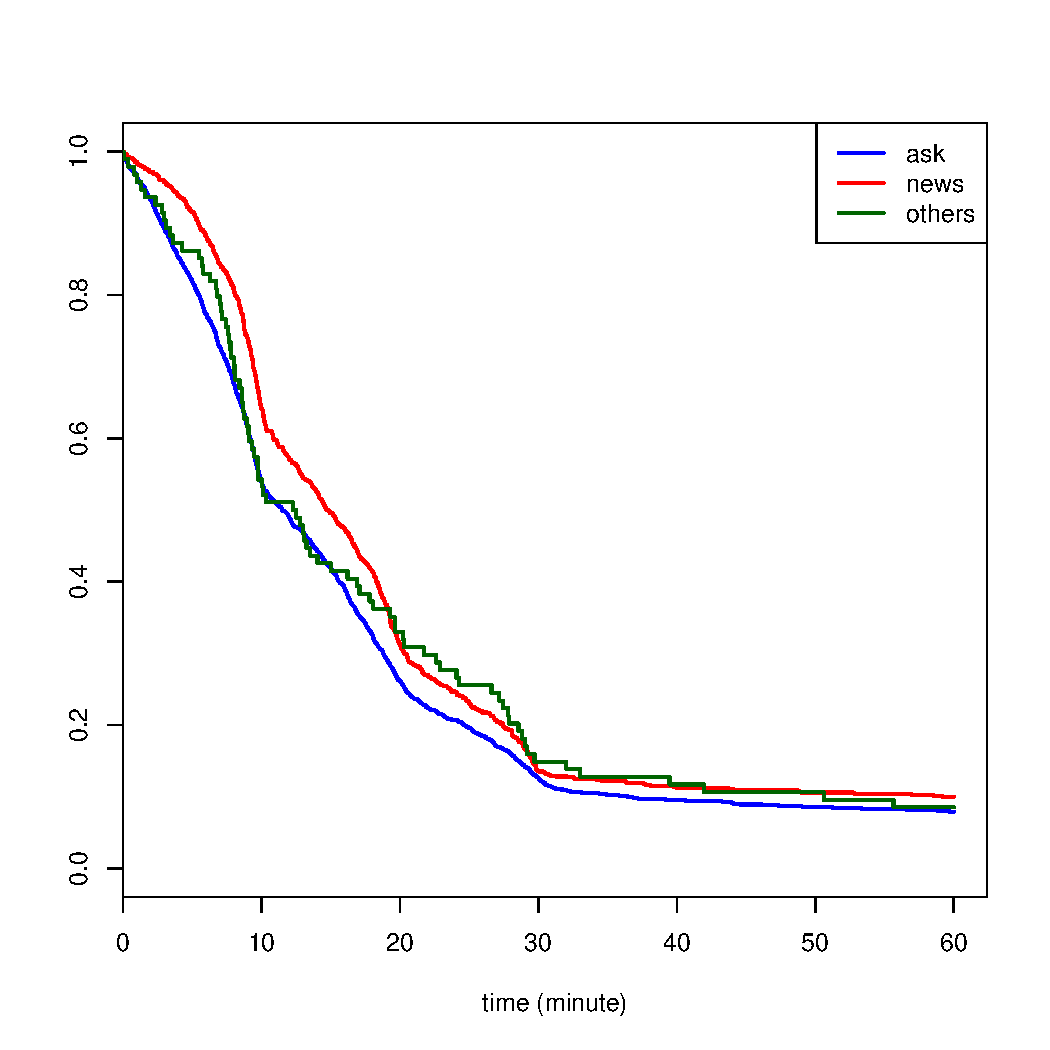
\includegraphics[width = .68\textwidth]{Figure/fig_cls_KM.pdf}
}

\frame{
\frametitle{Kaplan-Meier Estimate of Original Articles and Replyings}
\centering
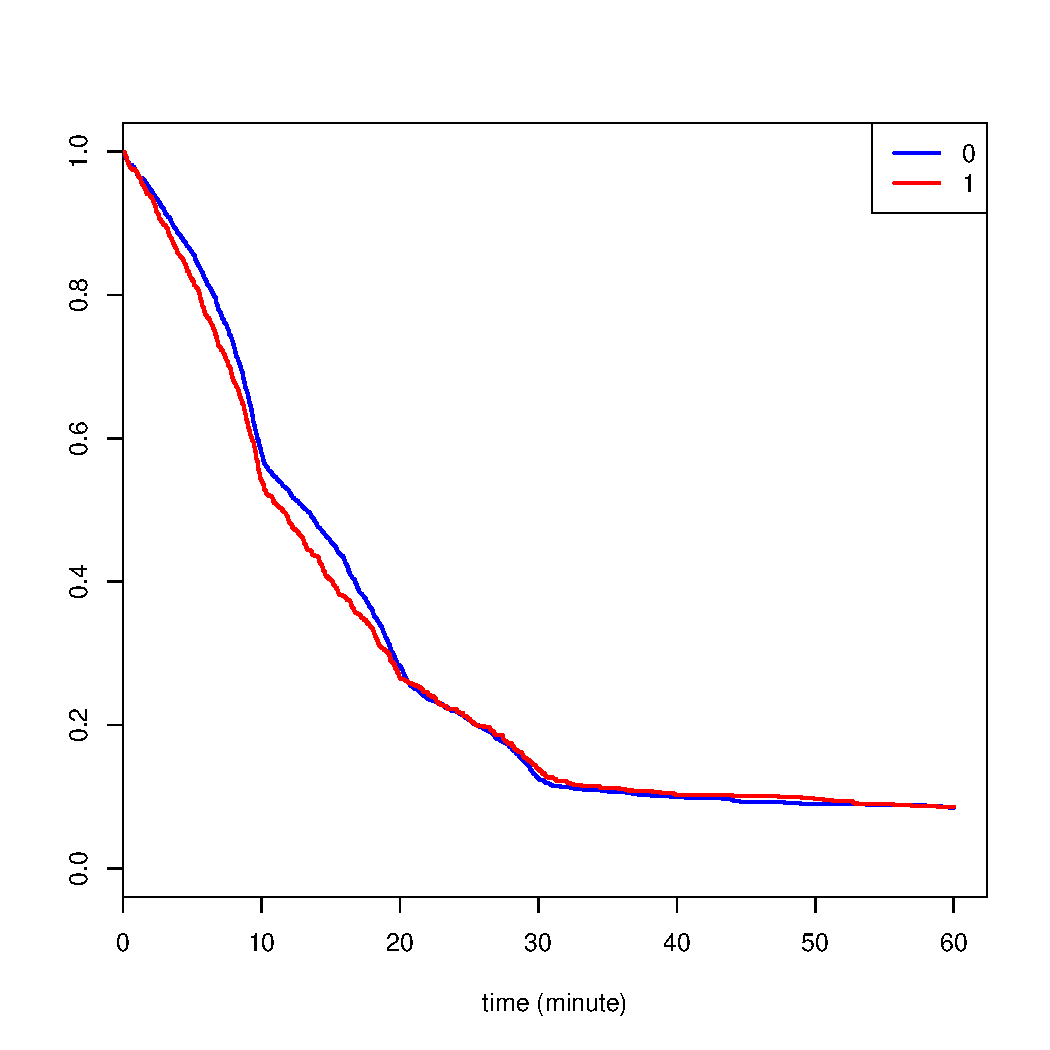
\includegraphics[width = .68\textwidth]{Figure/fig_re_KM.pdf}
}

\frame{
\frametitle{Kaplan-Meier Estimate with Evening}
\centering
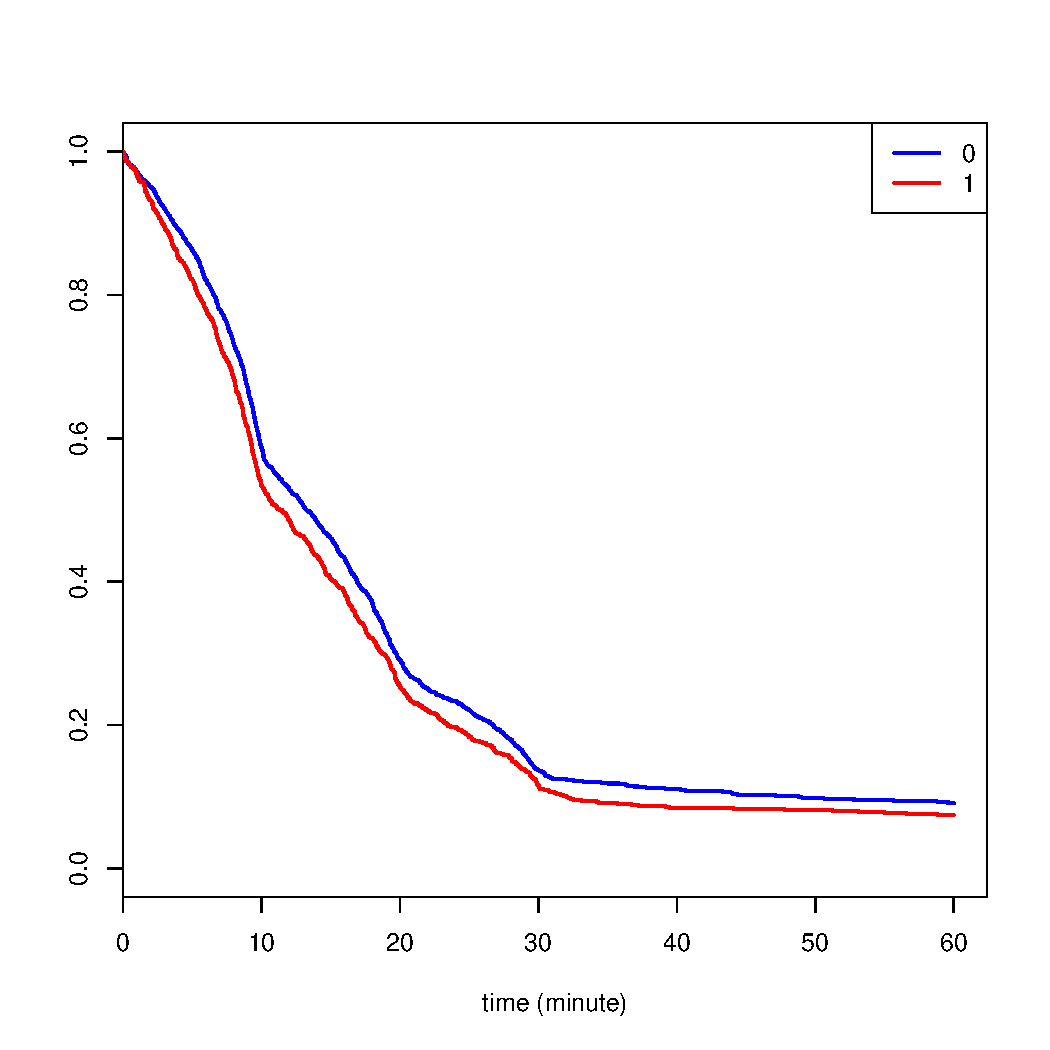
\includegraphics[width = .68\textwidth]{Figure/fig_Evening_KM.pdf}
}

\frame{
\frametitle{Kaplan-Meier Estimate with Weekend}
\centering
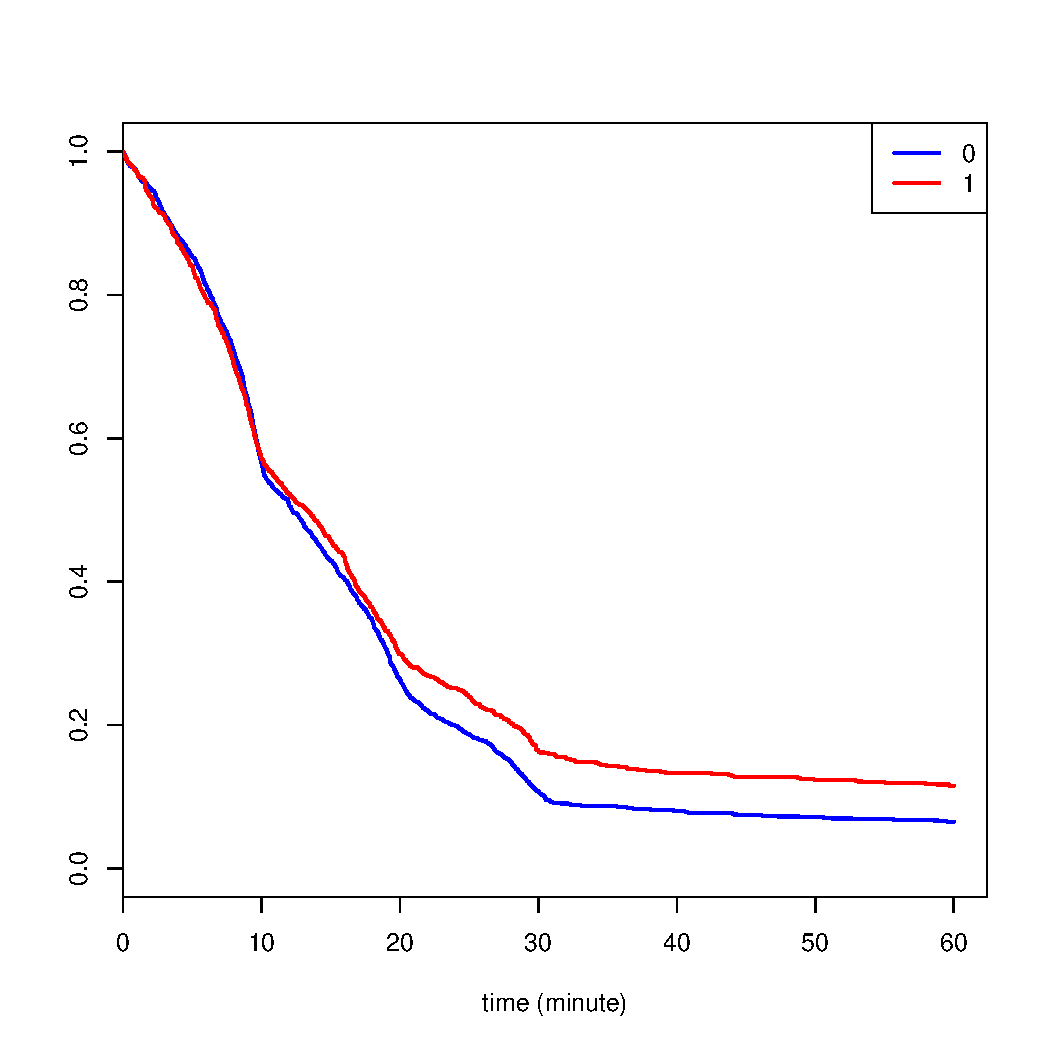
\includegraphics[width = .68\textwidth]{Figure/fig_weekend_KM.pdf}
}

\frame{
\frametitle{Kaplan-Meier Estimate with Graphs}
\centering
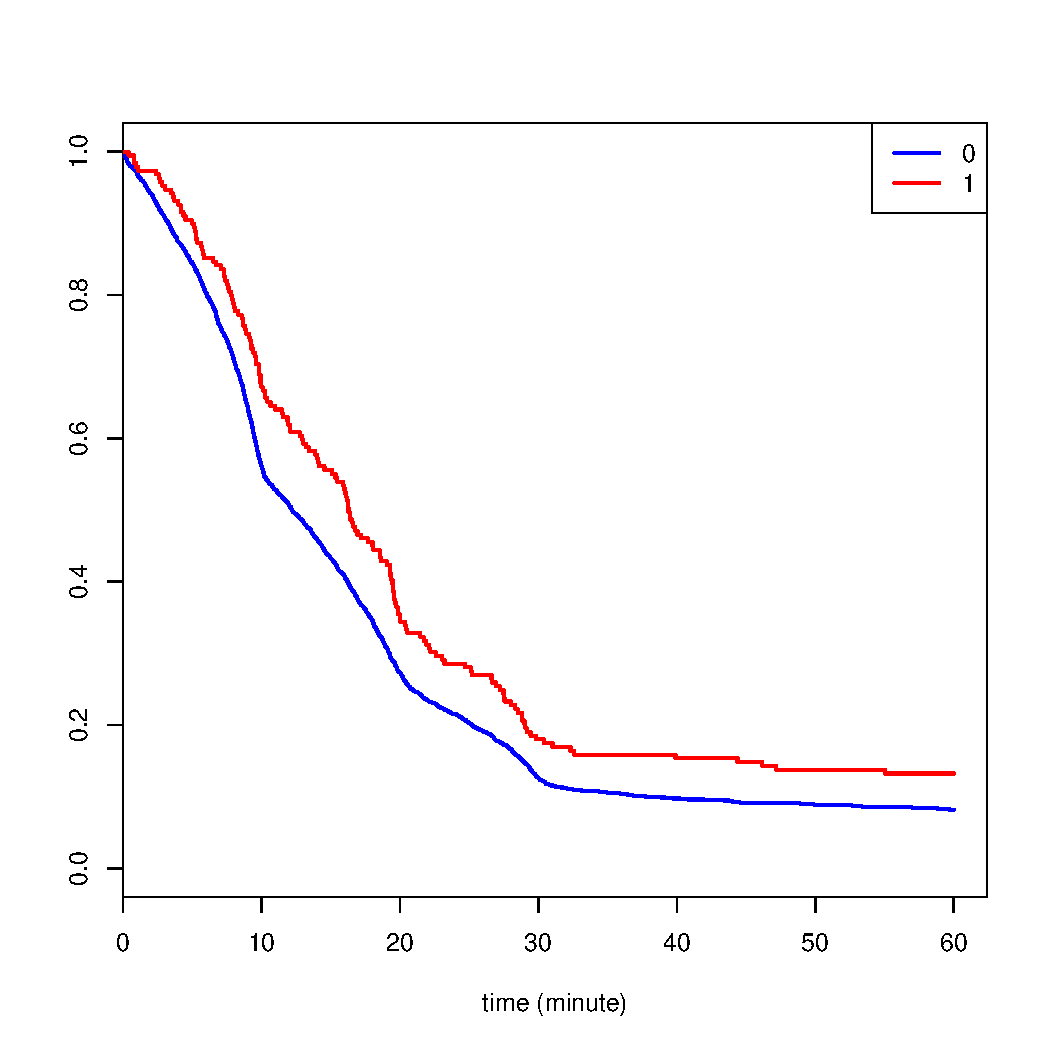
\includegraphics[width = .68\textwidth]{Figure/fig_graphId_KM.pdf}
}

\frame{
\frametitle{Kaplan-Meier Estimate with URL}
\centering
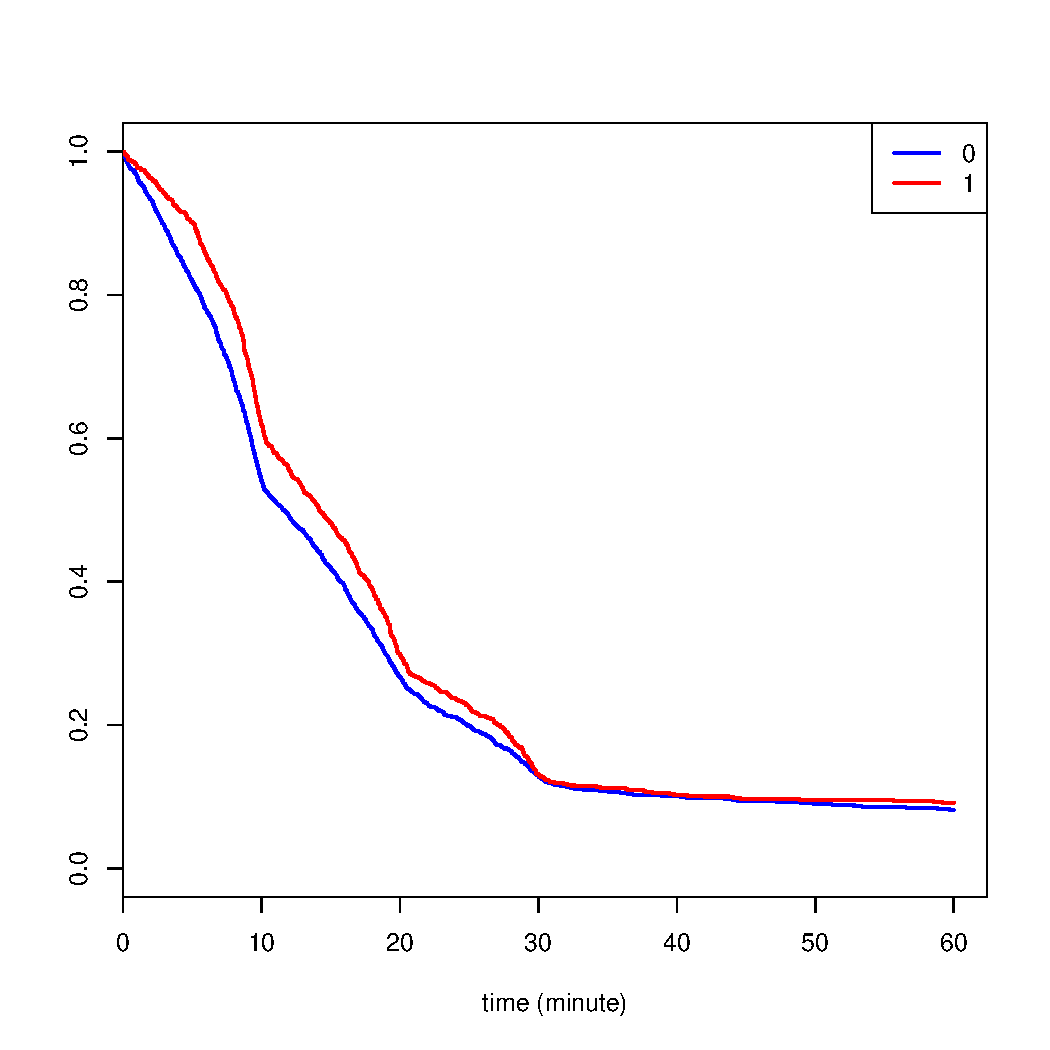
\includegraphics[width = .68\textwidth]{Figure/fig_httpId_KM.pdf}
}

\frame{
\frametitle{Kaplan-Meier Estimate with YouTube Link}
\centering
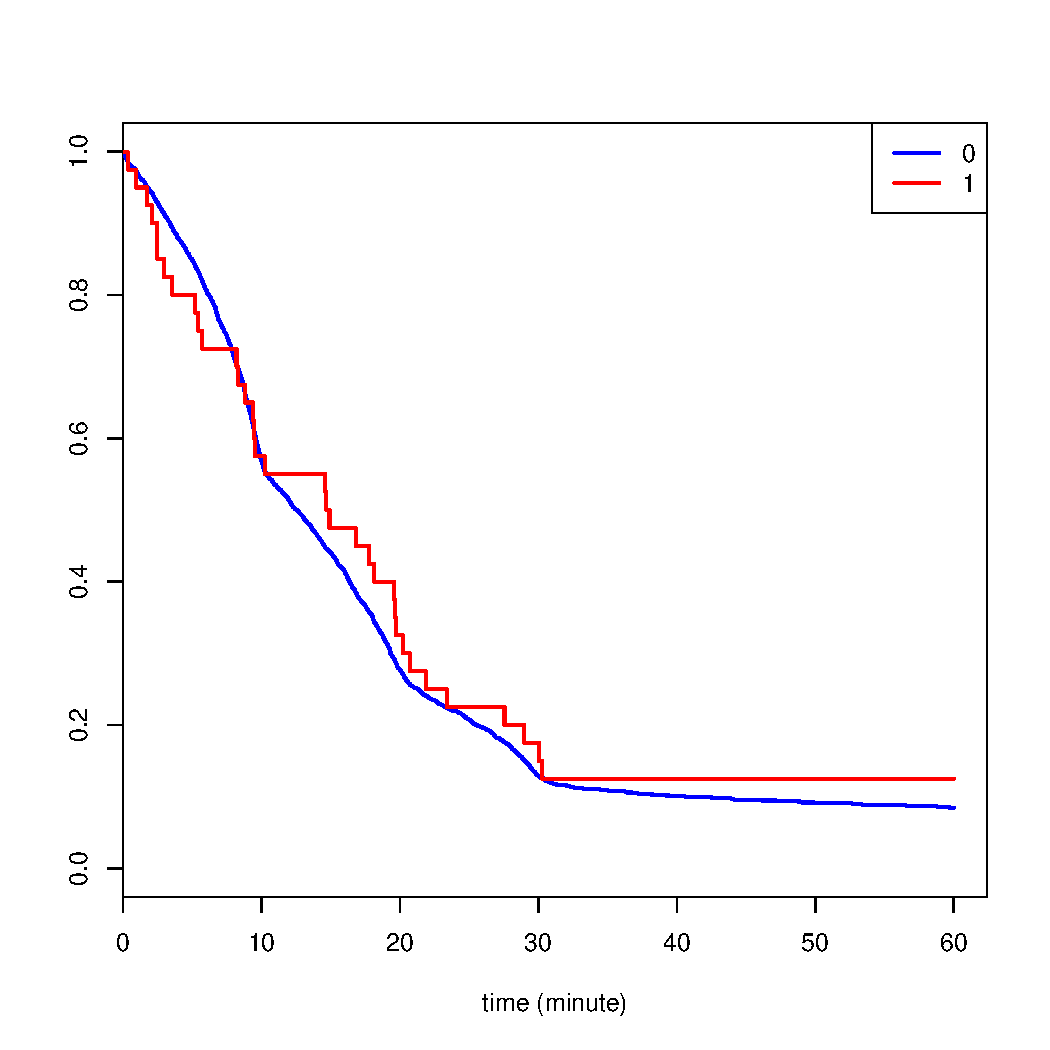
\includegraphics[width = .68\textwidth]{Figure/fig_youtubeId_KM.pdf}
}

\frame{
\frametitle{Kaplan-Meier Estimate with Garbage}
\centering
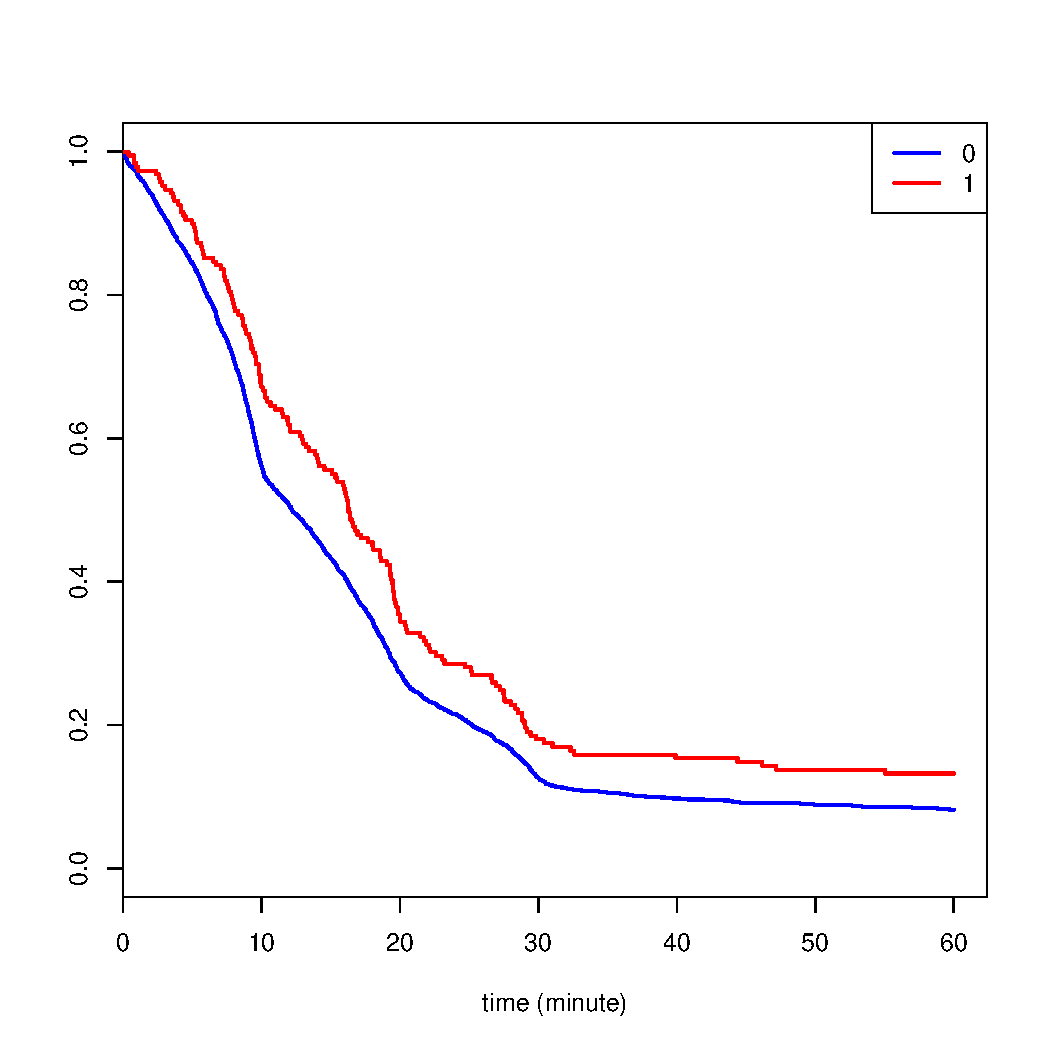
\includegraphics[width = .68\textwidth]{Figure/fig_garbage_KM.pdf}
}


\frame{
\frametitle{Fitting Distributions}
\centering
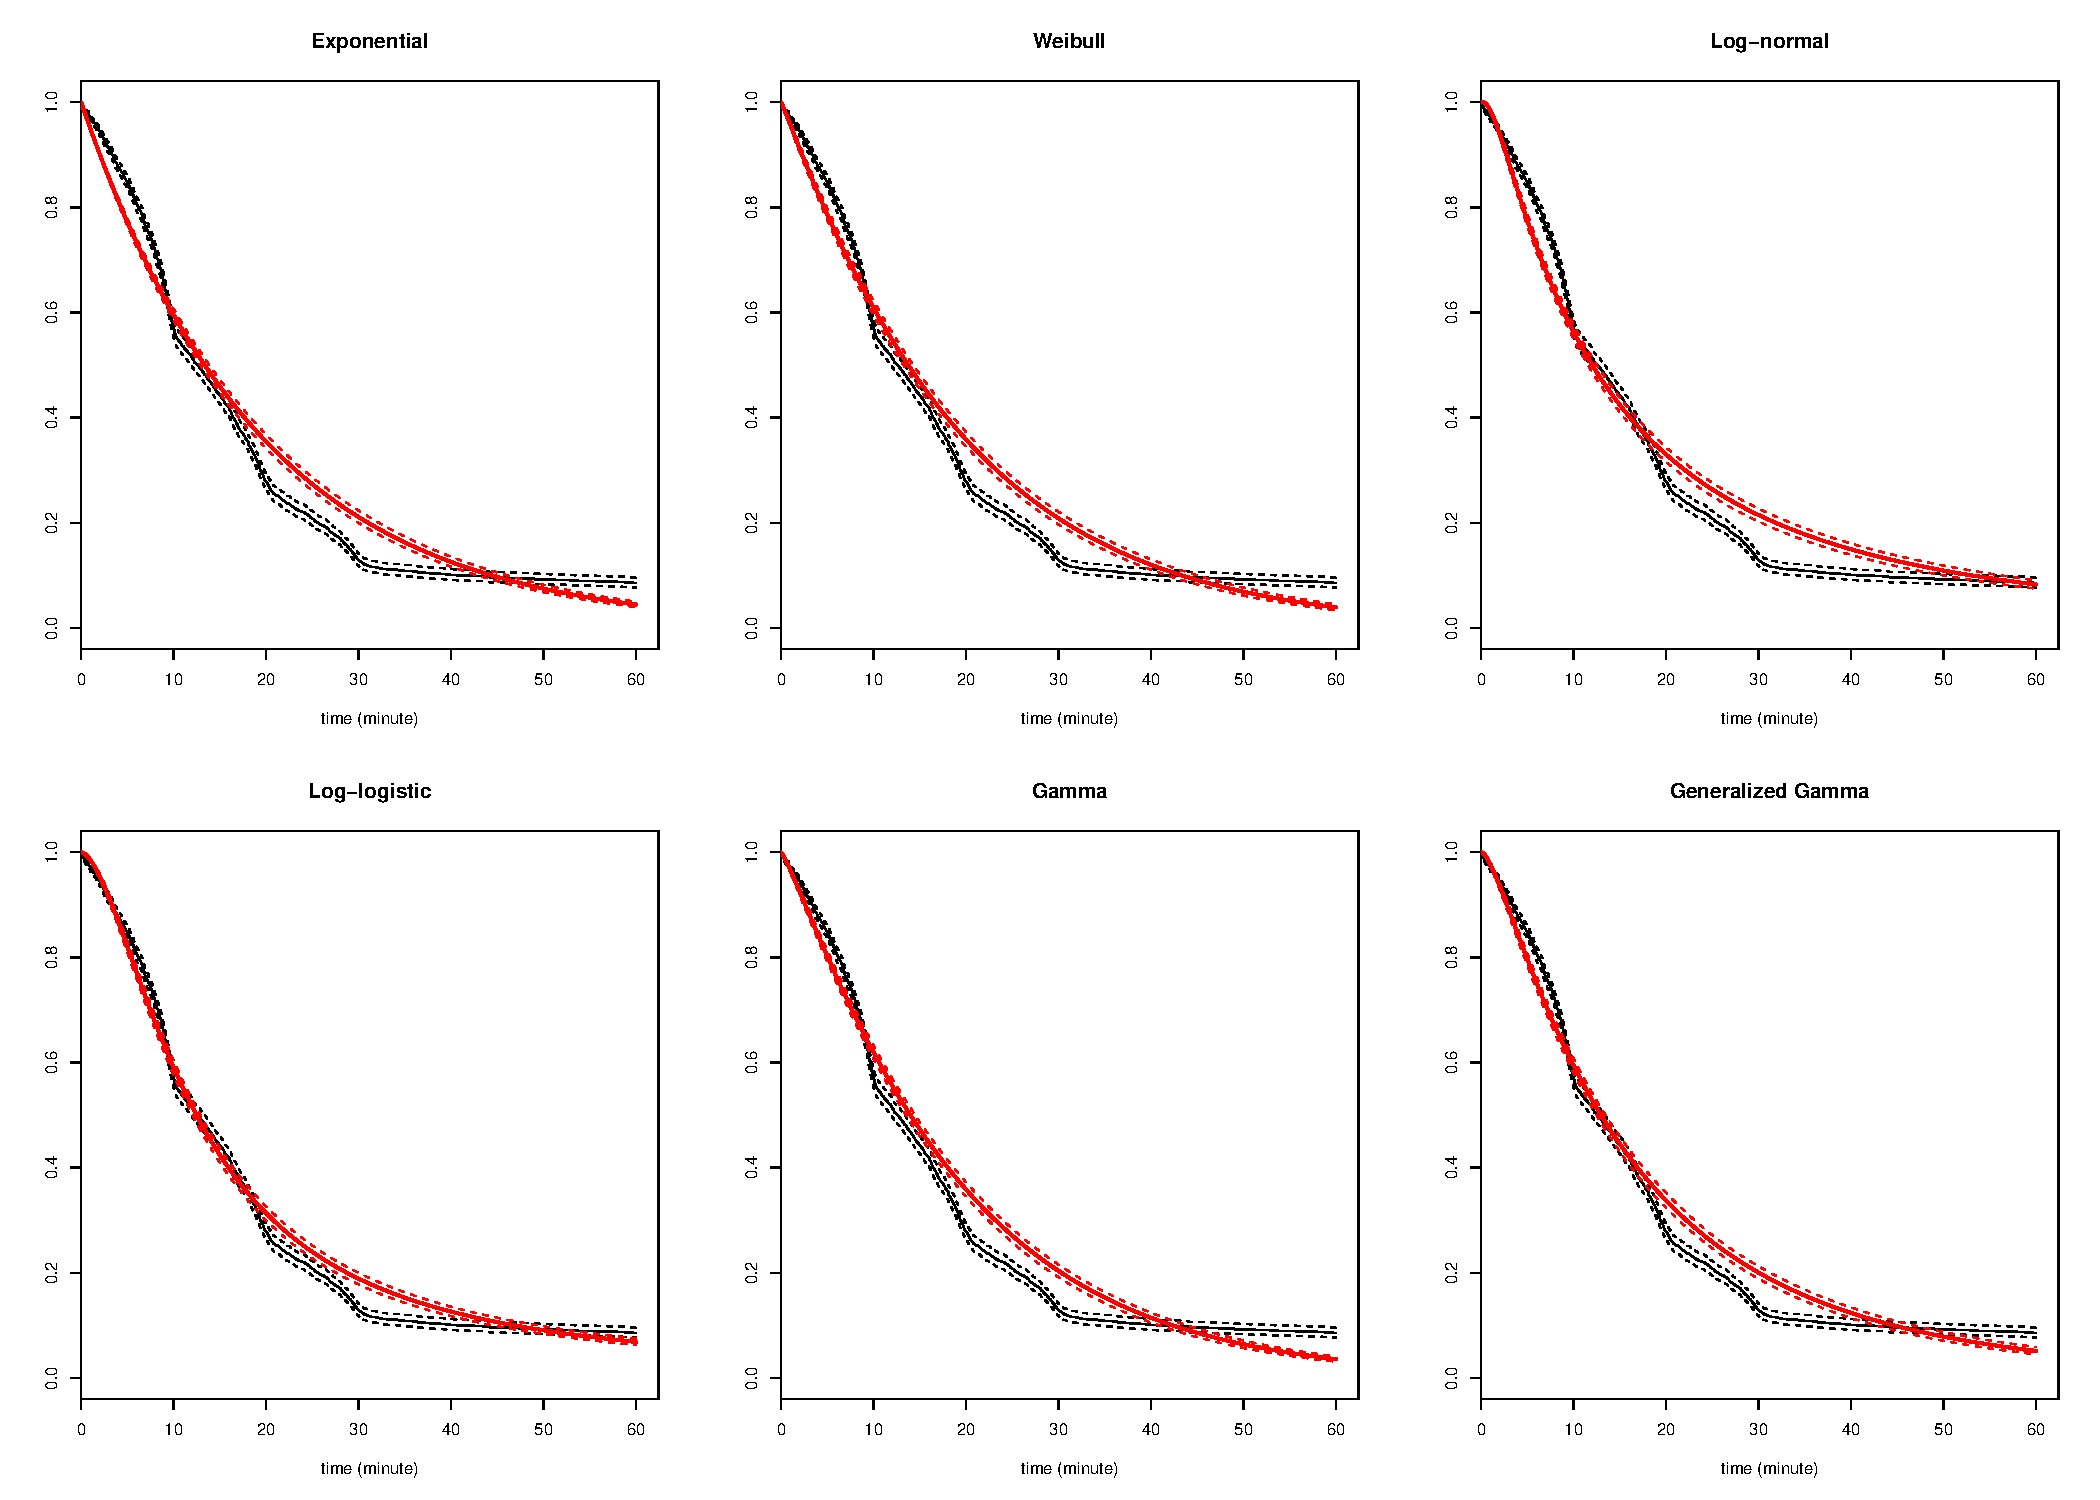
\includegraphics[width = .9\textwidth]{Figure/fig_survfit_dist.pdf}
}

\frame{
\frametitle{Fitting Distributions (cont.)}
\begin{table}[htp]
\caption{Distribution Fitting}
\begin{center}
\begin{tabular}{l | cc}
Distribution			&	AIC				&	loglikelihood		\\ \hline
Exponential 			&     	48934.04 			&	-24466.02			\\
Weibull           			&	48926.46 			&	-24461.23			\\
Log-normal       			&	48977.28 			&	-24486.64			\\
Log-logistic      			&	\alert{48571.03} 	&	\alert{-24283.51}	\\	
Gamma            			&	48895.46 			&	-24445.73			\\
Generalized Gamma 	&	48770.73 			&	-24382.37	
\end{tabular}
\end{center}
\label{default}
\end{table}%
}

\frame{
\frametitle{Cox PH Model}
\begin{table}[htp]
\caption{Coefficients of Covariates of the Original Model}
\begin{center}
\begin{tabular}{l | rrrl}
Covariate		&	Coef		&	exp(Coef)	&	p-value 	&	\\ \hline
Class: News  	&	-0.1760    	&	0.8386   	&	0.0038 	&	**	\\
Class: Others 	&	-0.0865  	&	0.9171 	&	0.4444 	&		\\
Reply          	&	0.0906    	&	1.0949  	&	0.0481 	&	*	\\
Evening        	&	0.1502    	&	1.1621   	&	0.0002 	&	***	\\
Weekend       	&	-0.1741    	&	0.8402   	&	0.0000 	&	***	\\
With Graphs     	&	-0.0166    	&	0.9836   	&	0.8329 	&		\\
With URL         	&	0.0247    	&	1.0250   	&	0.7243 	&		\\
Youtube Link    	&	-0.0873    	&	0.9164   	&	0.6217 	&		\\
Garbage    	&	-0.2375    	&	0.7886   	&	0.0033 	&	**	\\
Content Length	&	-0.0001    	&	0.9999   	&	0.0679 	&	.	\\
Policy Score   	&	0.7804    	&	2.1822   	&	0.3354	&	
\end{tabular}
\end{center}
\label{default}
\end{table}%
}


\frame{
\frametitle{Cox PH Model with Mixture Stepwise Selection}
\begin{table}[htp]
\caption{Coefficients of Covariates of the Original Model}
\begin{center}
\begin{tabular}{l | rrrl}
Covariate		&	Coef		&	exp(Coef)	&	p-value 	&		\\ \hline
Class: News   	&	-0.1565    	&	0.8551   	&	0.0009 	&	***	\\
Class: Others  	&	-0.0843    	&	0.9192   	&	0.4511 	&		\\
Reply         	&	0.0877    	&	1.0916   	&	0.0454 	&	*	\\
Evening      	&	0.1500    	&	1.1619   	&	0.0002 	&	***	\\
Weekend       	&	-0.1745    	&	0.8399   	&	0.0000 	&	***	\\
Garbage       	&	-0.2412    	&	0.7857   	&	0.0028 	&	**	\\
Content Length	&	-0.0001    	&	0.9999   	&	0.0637 	&	.	\\
\end{tabular}
\end{center}
\label{default}
\end{table}%
}

%%%%%%%%%%%%%%%%%%%%%%%%%%%%%%%%%%%%%%%%%%%%%%%%%%%%

\end{document}